\documentclass[10pt]{article}
\usepackage{icmlko}

\icmlmeta{IP 파운데이션 월드모델}{72}{자를 바꾸고 처음 한 일은 되돌리기였다}{판정치를 앙상블로 전환하고, 네 씨앗으로 확인한 뒤, 노트 48의 배선을 되돌린다}

\begin{document}

\twocolumn[
\icmlheader

\begin{abstract}
노트 71이 판정치를 바꿔야 한다고 했다. 바꿨다 --- 파이프라인이 이제 \textbf{앙상블
$\rho$를 앞에 세우고} 셀 평균을 괄호에 둔다. 구간도 두 자로 붙는다(앙상블 반폭
0.0453, 셀 평균 0.0321). 새 자로 처음 한 일이 \textbf{되돌리기}다. 노트 48이
웹툰 굿즈 규모를 연재 밀도에서 참여 작가 수로 바꿨는데, 새 자로 재면 되돌리는
쪽이 채택이다($+$0.0132 {[}$+$0.0005, $+$0.0313{]}). \textbf{효과가 문턱 바로
위라} 노트 67의 교훈대로 씨앗을 넷으로 늘려 확인했고 \textbf{4/4 채택}이라
적용했다 --- 문턱 근처 결정은 씨앗을 바꿔 확인한다는 규약을 새로 둔다. 적용
결과 앙상블 판정치가 $+$0.2612에서 \textbf{$+$0.2744}로, 웹툰 자기 상관이
$+$0.401에서 \textbf{$+$0.480}으로 오른다. \textbf{그런데 팝업은 $+$0.469에서
$+$0.459로 내렸다} --- 노트 38 · 40의 상충 법칙이고, 판정치와 제품 목표 사이에
아직 남은 간극이다. 방향 결정도 마저 정리했다. 세 순서 중 \textbf{부호 뒤
합치기}가 최선이지만($k{=}32$에서 $+$0.3212) 셋 다 채택 문턱에 못 간다. 이유가
좋다 --- \textbf{앙상블이 이미 오정향의 절반을 흡수한다.} 방향 틀린 도메인
하나의 값이 셀 평균에서 $-$0.1772이고 앙상블에서 $-$0.1027로, \textbf{42\%
싸다}.
\end{abstract}
]

\begin{figure*}[t]
\centering
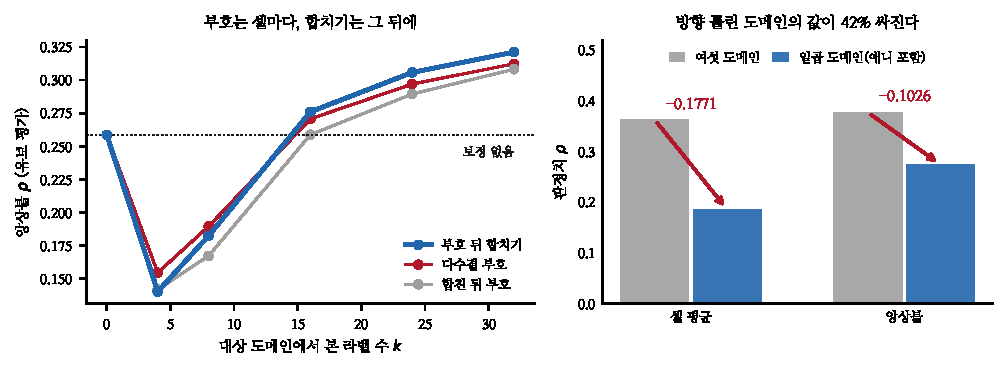
\includegraphics[width=\textwidth]{figs/metric.pdf}
\caption{왼쪽 --- 부호와 합치기의 순서. 오른쪽 --- 방향 틀린 도메인의 값.}
\end{figure*}

\section{자를 갈아 끼웠다}

\texttt{state/pipeline.py}가 이제 앙상블을 앞에 세운다. \texttt{state/audit.py}에
\texttt{rho\_ens}를 넣어 모든 판정을 두 자로 잴 수 있다.

\begin{table}[t]
\centering\tsize
\caption{두 자로 잰 구간. 붓스트랩 150회.}
\begin{tabular}{lrrl}
\toprule
& $\rho$ & 반폭 & 95\% 구간 \\
\midrule
\textbf{앙상블} & \textbf{$+$0.2744} & 0.0453 & $[+0.212, +0.303]$ \\
셀 평균 & $+$0.1858 & 0.0321 & $[+0.137, +0.202]$ \\
\bottomrule
\end{tabular}
\end{table}

앙상블 쪽 구간이 절대값으로는 넓지만 상대 폭은 같다(16.5\% 대 17.3\%). 재는
값이 더 크고 더 뜻이 있으므로 이쪽을 정본으로 둔다.

\section{되돌리기}

\begin{table}[t]
\centering\tsize
\caption{웹툰 굿즈 규모를 연재 밀도로 되돌리기. 붓스트랩 300회.}
\begin{tabular}{lrl}
\toprule
씨앗 & $\Delta$ & 95\% 구간 \\
\midrule
20260729 & $+$0.0132 & $[+0.0005, +0.0313]$ \\
19770101 & $+$0.0132 & $[+0.0035, +0.0305]$ \\
20250315 & $+$0.0132 & $[+0.0022, +0.0329]$ \\
20260101 & $+$0.0132 & $[+0.0028, +0.0298]$ \\
\midrule
\multicolumn{2}{l}{셀 평균 자로(참고)} & 보류 \\
\bottomrule
\end{tabular}
\end{table}

첫 씨앗의 하한이 $+$0.0005다. 이 정도면 씨앗 하나로 판정할 수 없다.

\claimx{판정 문턱 근처(하한이 0.005 미만)의 결정은 씨앗을 넷으로 늘려 전부
통과할 때만 적용한다. 노트 67이 ``작은 표본에서 고른 배선이 큰 표본에서 사라진다''를
보였고, 같은 위험이 붓스트랩 씨앗에도 있다.}{씨앗 넷도 임의의 수다. 넷이 전부
같은 데이터에서 뽑히므로 표본 자체의 편향은 못 잡는다.}

적용했다. 노트 46이 골랐고 노트 48이 바꿨고 노트 67이 무효화했고 노트 72가
되돌린 배선이다.

\begin{table}[t]
\centering\tsize
\caption{되돌린 뒤.}
\begin{tabular}{lrr}
\toprule
& 전 & 후 \\
\midrule
앙상블 판정치 & $+$0.2612 & \textbf{$+$0.2744} \\
셀 평균 & $+$0.1797 & $+$0.1858 \\
웹툰 자기 $\rho$ & $+$0.401 & \textbf{$+$0.480} \\
웹툰 앙상블 & $+$0.395 & $+$0.482 \\
\textbf{팝업 앙상블} & \textbf{$+$0.469} & \textbf{$+$0.459} \\
\bottomrule
\end{tabular}
\end{table}

\paragraph{팝업이 내렸다}
웹툰이 크게 오르고 팝업이 조금 내린다. 노트 38 · 40의 상충 법칙 그대로다 ---
한 도메인의 자기 상관을 올리면 그 도메인은 대상으로 좋아지고 출처로 나빠진다.
웹툰은 팝업의 출처 중 하나다.

\begin{quote}\fontsize{9.5}{11.5}\selectfont
\textbf{판정치와 제품 목표는 아직 다르다.} 일곱 대상 평균은 올랐고 팝업 하나는
내렸다. 팝업만 보고 고르면 75건에 과적합하므로 평균을 쓰는데, 그 대가가 이런
경우다. 지금은 평균을 따르되 팝업이 내려간 것을 기록해 둔다.
\end{quote}

\section{방향 결정 --- 부호는 셀마다, 합치기는 그 뒤에}

\begin{table}[t]
\centering\tsize
\caption{앙상블 $\rho$(유보 평가). 복제 150회.}
\begin{tabular}{lrrr}
\toprule
$k$ & 합친 뒤 부호 & 다수결 & 부호 뒤 합치기 \\
\midrule
0 & $+$0.2586 & $+$0.2586 & $+$0.2586 \\
8 & $+$0.1671 & $+$0.1894 & $+$0.1823 \\
16 & $+$0.2587 & $+$0.2707 & $+$0.2760 \\
24 & $+$0.2895 & $+$0.2970 & $+$0.3058 \\
\textbf{32} & $+$0.3082 & $+$0.3123 & \textbf{$+$0.3212} \\
\bottomrule
\end{tabular}
\end{table}

순서가 $k\ge16$에서 일관된다 --- \textbf{부호 뒤 합치기 $>$ 다수결 $>$ 합친 뒤
부호}. 결정은 셀마다 여섯 번 하고(헤지) 예측은 합치는(이득) 조합이 맞다.
그런데 셋 다 짝지은 구간이 0을 포함한다($k{=}32$에서 $+$0.0626 {[}$-$0.051,
$+$0.104{]}).

\section{앙상블이 이미 절반을 흡수한다}

\begin{table}[t]
\centering\tsize
\caption{방향 틀린 도메인(애니) 하나를 넣는 값.}
\begin{tabular}{lrrr}
\toprule
& 6도메인 & 7도메인 & 값 \\
\midrule
셀 평균 & $+$0.3629 & $+$0.1858 & $-$0.1772 \\
\textbf{앙상블} & $+$0.3770 & $+$0.2744 & \textbf{$-$0.1027} \\
\bottomrule
\end{tabular}
\end{table}

\claimx{앙상블은 방향 틀린 도메인의 값을 42\% 깎는다. 셀 평균에서는 그 도메인이
대상으로도 출처로도 매번 온전히 값을 치르는데, 앙상블에서는 출처일 때 여섯 중
하나로 희석되고 대상일 때만 온전히 치른다.}{애니 하나로 잰 비율이다. 방향 틀린
도메인이 둘이면 희석이 덜 될 것이다.}

이것이 방향 보정이 채택 문턱에 못 가는 이유이기도 하다. 고칠 손상이 이미 절반으로
줄어 있으니 고쳐서 얻을 것도 절반이다.

\section{한계}

\begin{itemize}[leftmargin=1.1em,itemsep=0.15em]
\item 판정치를 바꿨으니 노트 33 이후 결정 전부가 원칙적으로 재검토 대상인데
      다섯 개만 다시 쟀다.
\item 팝업 앙상블이 내려간 것을 ``평균이 올랐으니 채택''으로 넘겼다. 제품
      관점에서는 틀린 선택일 수 있다.
\item 씨앗 넷 규약을 이번 한 결정에만 썼다. 소급 적용은 안 했다.
\item 방향 보정을 여전히 정본에 안 넣었다 --- 세 순서 중 최선을 골랐으나 채택
      문턱을 못 넘었다.
\item 애니가 방향이 뒤집힌 채로 판정치에 들어가 있다. 앙상블이 값을 깎아 주지만
      $-$0.1027은 여전히 크다.
\end{itemize}

\section{다음}

\begin{enumerate}[leftmargin=1.3em,itemsep=0.15em]
\item 여덟째 도메인. 앙상블은 출처가 많을수록 유리하므로 셀 평균으로 볼 때보다
      값이 크다.
\item 팝업만을 목표로 한 판정치를 따로 만들어 본다 --- 일곱 평균과 얼마나
      갈리는지.
\item 앙상블 가중치를 라벨 몇 건으로 정해 본다. 부호가 $\pm1$ 가중치의 특수한
      경우이므로 연속 가중치가 자연스러운 일반화다.
\item 노트 34 도서 배선 등 남은 과거 결정을 새 자로 다시 잰다.
\end{enumerate}

\vspace{0.6em}
\hrule height 0.3pt
\vspace{0.5em}
{\footnotesize
\textbf{참고문헌}\\[0.3em]
Breiman, L. (1996). Bagging predictors. \emph{Machine Learning}, 24(2), 123--140.\\[0.15em]
Kuncheva, L. I., Whitaker, C. J. (2003). Measures of diversity in classifier
ensembles. \emph{Machine Learning}, 51(2), 181--207.\\[0.15em]
Cawley, G. C., Talbot, N. L. C. (2010). On over-fitting in model selection and
subsequent selection bias in performance evaluation. \emph{JMLR}, 11, 2079--2107.\\[0.15em]
Bouthillier, X. et al. (2021). Accounting for variance in machine learning
benchmarks. \emph{MLSys}, 3, 747--769.\\[0.15em]
Efron, B., Tibshirani, R. J. (1993). \emph{An Introduction to the Bootstrap}.
Chapman \& Hall.
}

\end{document}
